\documentclass{article}

% --- load packages ---

\usepackage[margin=1.5in]{geometry} % change the margins
\usepackage{amsmath} % useful math environments and commands like align
\usepackage[colorlinks,bookmarks,bookmarksnumbered,allcolors=blue]{hyperref} % hyperlinks between references
\usepackage{graphicx}  % include images
\usepackage[caption=false]{subfig} % subfigures.  false option prevents conflicts in caption styling with other packages
\usepackage{booktabs} % better tables
\usepackage[capitalise]{cleveref} % better referencing. uses cref.
\usepackage[section]{placeins} % sometimes useful to prevent figures from floating out of a section
\usepackage{cite} % handles multiple citations in one command better
\usepackage{doi} % allow correct hypderlinking of DOIs

% Added by me
\usepackage[labelfont=bf]{caption}
\usepackage{siunitx}
\usepackage[sc]{mathpazo}
\usepackage{amsmath,mathtools,amssymb}
\usepackage{unicode-math}
\usepackage{footnote}
\makesavenoteenv{tabular}
\makesavenoteenv{table}

\DeclarePairedDelimiter{\norm}{\lVert}{\rVert}
\DeclareRobustCommand\widebar[1]{\mathop{\overline{#1}}}

% Back to template
\begin{document}

\title{ME 575 --- Homework 3}
\author{Seth Nielsen}
% put in \date{} if you don't want a date to appear, or enter a specific date, otherwise default is today's date.
\date{}
\maketitle

\section*{Introduction}

For this assignment, I worked on optimizing the same 10-bar truss problem from the first homework, but with the gradients for the objective and the contraints provided by my own algorithms. I did the assignment entirely in Python 3. The following four approaches were used for computing the gradients:

\begin{enumerate}
	\item Forward-difference
	\item Complex-step
	\item Forward-mode autodifferentiation (provided by Google's \texttt{JAX} library)
	\item Analytic adjoint
\end{enumerate}

\section{Truss Derivatives}

Let $A$ be the array containing the cross-sectional areas of the ten bars that make up the truss. Let $m$ be the total mass of the truss. Let $\sigma$ be the array containing the stress on each of the ten bars. The derivatives calculated by each of the four methods were:
\begin{itemize}
	\item $ \displaystyle \frac{dm}{dA} $ --- mass with respect to each cross-sectional area (array of size 10)
	\item $ \displaystyle \frac{d\sigma}{dA} $ --- all stresses with respect to each cross-sectional area (2D-array of size 10$\times$10)
\end{itemize}
After successfully computing the derivatives using each method, the results of each were analyzed. I computed the relative differences of each result using several different measures, which are outlined below. Of the four methods, the derivatives obtained through the analytic adjoint method were chosen to be the `true' values that the derivatives from the other methods were compared against. For the ensuing error analysis, let $d$ be the correct derivative value (as computed by the adjoint method) of one of the two derivatives of interest. Let $\hat{d}$ be the derivative value computed by one of the other three methods. With those definitions, we can now attempt to analyze the relative error of each result. The following three distinct measures were chosen to express the relative error: 
\begin{enumerate}
	\item The $L_2$ norm of the difference of the gradient computed by each method where a value of 1 in$^2$ was assigned to all cross-sectional areas, which will be denoted as 
	\begin{equation*}
		E_{1} = \norm{ \hat{d} - d }_2
	\end{equation*}
	\item The $L_2$ norm of the average difference of the gradients computed at 100 uniformly random evaluation points (i.e., 100 arrays of unique values for areas) generated over the interval $[0.1, 2.0)$, which will be denoted as
	\begin{equation*}
		\bar{E} = \norm{ ( \widebar{ \hat{d} - d } ) }_2
	\end{equation*}
	\item Same as 2, but instead contains the maximum element taken from the gradient difference at their respective positions in the resulting vector (mass gradient) or matrix (stresses gradient), which can be expressed as 
	\begin{equation*}
		E_{\max} = \norm{ \max_{i}( \hat{d} - d ) }_2
	\end{equation*}

\end{enumerate}
% 
The relative errors for the different methods are displayed in Tables~\ref{tab:ones}-\ref{tab:max}.

\footnotetext[1]{To within 30 digits of precision}

\begin{table}[htb]
	\centering
	\caption{Comparison of relative error $E_{1}$ for each area $a_i = 1\text{ in}^2$}\label{tab:ones}
	\begin{tabular}{r c c c}
		\toprule
		\textbf{Property} & Forward-difference & Complex-step & Autodifferentiation \\
		\midrule
		\textbf{mass (lb)} & 7.39109753e-06 & 0.0\footnotemark[1] & 0.0\footnotemark[1] \\
		\textbf{stress (psi)} & 2.71446719e-01 & 1.84318837e-09 & 2.95593665e-10 \\
		\bottomrule
	\end{tabular}
\end{table}


\begin{table}[htb]
	\centering
	\caption{Comparison of \textit{mean} relative error $\bar{E}$ for 100 random areas}\label{tab:mean}
	\begin{tabular}{r c c c}
		\toprule
		\textbf{Property} & Forward-difference & Complex-step & Autodifferentiation \\
		\midrule
		\textbf{mass (lb)} & 7.26401808e-07 & 0.0\footnotemark[1] & 0.0\footnotemark[1] \\
		\textbf{stress (psi)} & 4.15404514e-02 & 7.68644189e-10 & 1.64377792e-10 \\
		\bottomrule
	\end{tabular}
\end{table}


\begin{table}[htb]
	\centering
	\caption{Comparison of \textit{max} relative error $E_{\max}$ for 100 random areas}\label{tab:max}
	\begin{tabular}{r c c c}
		\toprule
		\textbf{Property} & Forward-difference & Complex-step & Autodifferentiation \\
		\midrule
		\textbf{mass (lb)} & 1.88570408e-05 & 0.0\footnotemark[1] & 0.0\footnotemark[1] \\
		\textbf{stress (psi)} & 1.97270024 & 2.71107938e-08 & 1.05571766e-08 \\
		\bottomrule
	\end{tabular}
\end{table}

From these results, it is clear that the method suffering from the greatest relative error is the forward-difference method. The result makes sense if it is taken into account the limits of machine precision and the loss of precision that occurs when differencing numbers of fixed-precision.

\section{Truss Optimization With Derivatives Supplied}

To perform the actual optimization, I used the Python library pyOptSparse and the SNOPT algorithm. To report the results of the optimization, the convergence plots in Figure~\ref{fig:converge} were generated. The optimization algorithms were ran with all truss elements initialized with an area of 1 in$^2$. 

The number of objective function evaluations required for convergence for both methods is summarized in Table~\ref{tab:evals}. From these results, it can be seen that not only is the adjoint method superior in accuracy to the finite difference method, but it also requires much fewer evaluations of the objective function (in this case, by an order of magnitude). The disadvantage, however, is that the adjoint method requires understanding the mathematical model of each system that is to be optimized, and so is not as easily applied from one optimization problem to another as the finite difference method is.

\begin{table}[htb]
	\centering
	\caption{The number of function evaluations required to converge}\label{tab:evals}
	\begin{tabular}{c c}
		\toprule
		\textbf{Method} & Mean function calls \\
		\midrule
		\textbf{forward-difference} & 249.5 \\
		\textbf{adjoint} & 28.95 \\ 
		\bottomrule
	\end{tabular}
\end{table}

\begin{figure}[htb]
	\centering
	% 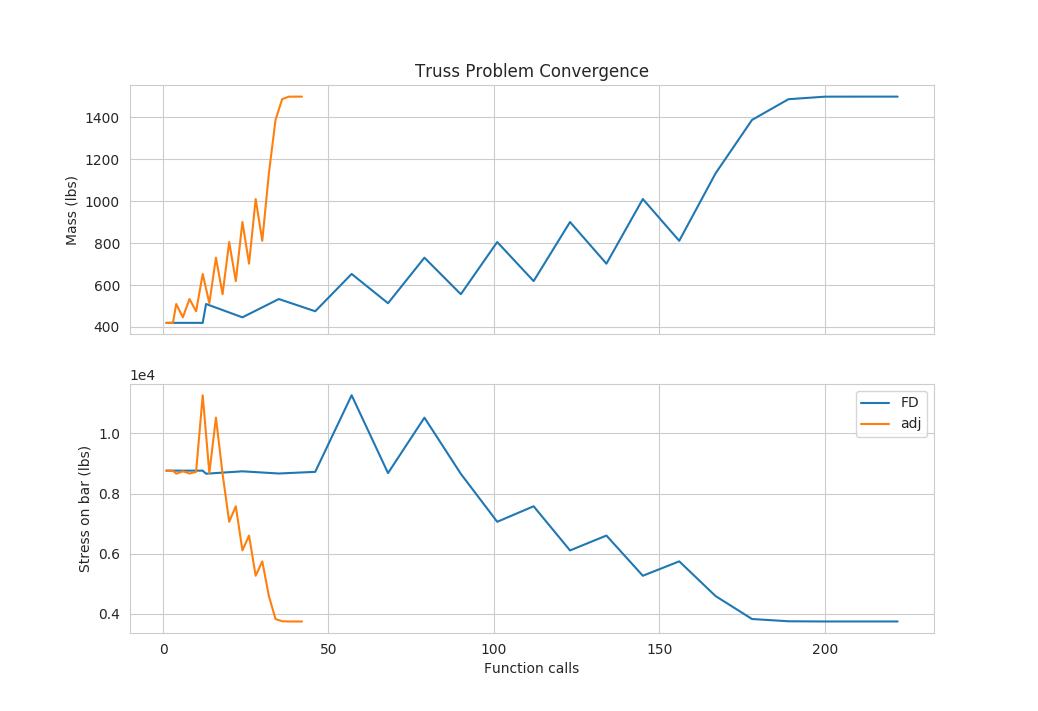
\includegraphics[width=0.75\textwidth]{figures/convergence.png}
	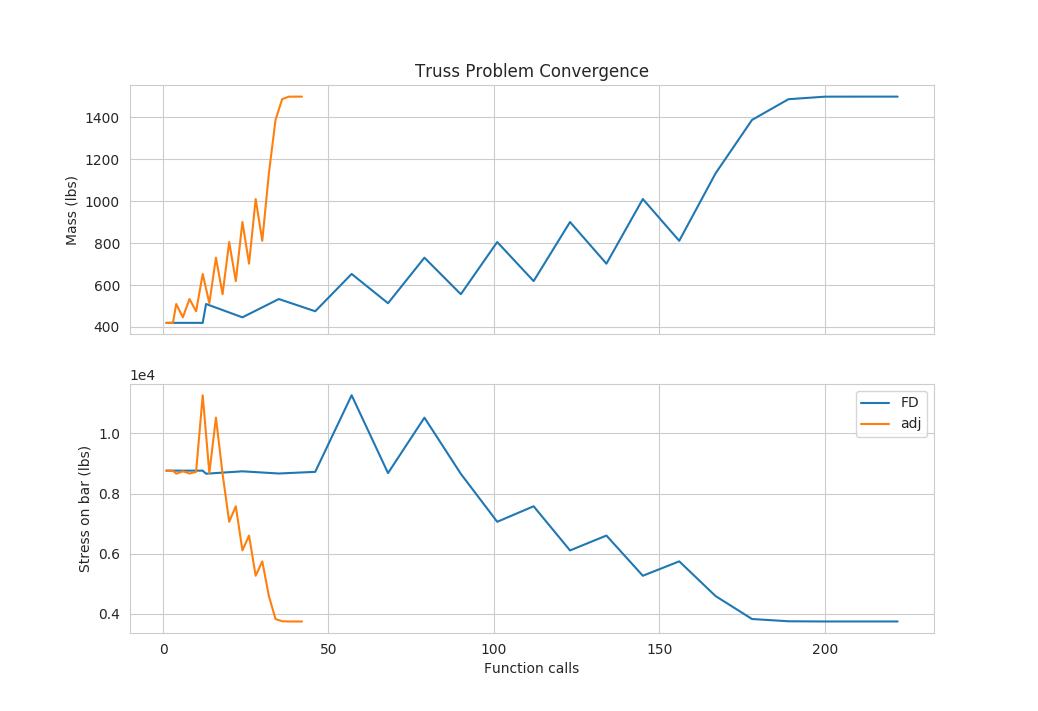
\includegraphics[width=\textwidth]{figures/convergence.png}
	\caption{Convergence plots for both the finite difference and adjoint methods.\label{fig:converge}}
\end{figure}


% This is for the bibliography.  Note that it is using sample.bib
% you would need to provide your own bibtex file.

\end{document}